\section{Implementation}
\label{sec:eval}

The implementation of the three algorithms for empirical results has been done using the C++ programming language along with the Message Passing Interface standard (MPI). The experiments were carried out using the infrastructure provided by SHARCNET. The 64 bit high performance Opteron and Xeon clusters, consisted of a maximum of 16 nodes, with upto 4 cores on each node. The clusters run the Linux Operating system and are interconnected with each other through a private, dedicated connection running at 10 Gigabits per second. The complete implementation has been written in approximately $2$K lines of code. The source code for the same can be found at https://github.com/shreya-68/Consensus/tree/master/MPI. The input into the system is a specified size of the network, i.e., total number of processes along with the input value for each of the processes for achieving consensus. The ratio of number of byzantine processes to the number of good processes is given as input as well along with a specified byzantine behavior. In accordand with this, the byzantine processes decide on which values to send at every round of the protocols. 

The output was the time taken (in the number of rounds), CPU time utilization, number of messages/bits sent per node, and the final decision value of each process. As a basic framework a synchronous peer-to-peer network was setup. On top of this network the algorithms were implemented for testing purposes.  

\subsection{Testing parameters}
For testing the three algorithms, we consider variable number of processes and variable number of faults. The number of processes $(n)$ ranges from $4$ to $64$. The number of faults $(f)$ lies in the range $[0, n/3)$ for algorithms Pull-Push and EIG, and in the range $[0, n/4)$ for algorithm Quorum. These ranges have been considered since the algorithms have been shown to be correct only in these respective ranges.

\subsection{Authentication of processes}
It was assumed that the channels are authenticated and each receiving entity knows the identity of the sender. The communication primitives provided by the MPI library implicitly provide this functionality and hence, a byzantine process cannot spoof their identity or hide it.

\subsection{Connection}
Each process in the peer-to-peer network had full knowledge about the network connection of other processes, i.e., the IP address and port number of the hosts it was connected to. Using the MPI library this is done by giving and ID to each node between and including $0$ and the size of the network. The MPI point-to-point operations were used for sending and receiving messages between two, and only two processes. This behaves like a TCP connection and was used for reliable transfer of messages between hosts. It also guarantees order between messages but does not guarantee fairness. The implementation does not make use any shared resources.

\subsection{Parallelization}
To allow programs to execute parts of the protocol that are independent of each other parallely, MPI thread level support has been used. In some cases non-blocking calls have been used, for example, if the execution of next few instructions does not depend on the completion of a send call then a non-blocking call is used. The MPI implementation creates a system buffer to typically hold data in transit. This is useful when a process wants to receive some messages sent to it by multiple other processes at a later time. This helped us improve performance to an extent since it allows for send-receive operation to be asynchronous. Nevertheless, it is a finite resource and should be used carefully otherwise it can lead to loss of messages. 

\subsection{Byzantine behaviors}
The byzantine behavior can be described in the following manner:
\begin{itemize}
    \item Crash failure: Processes may fail by stopping. Any good process that fails to send messages or aborts its execution is considered byzantine.
    \item Processes send conflicting data to different processes in the same round. Any data that is not the same or is null is said to be conflicting.
    \item Processes send arbitrary content or more messages than necessary. Byzantine processes may try to do so to choke the communication and flood the network or overload the requests that need to be answered.
    \item Denial of service: Byzantine processes may deny responding to requests from good processes or may not forward messages as required. 
\end{itemize}

\subsection{Synchronization}
To implement a synchronous model of communication, we make use of communicators, that is essentially a group of processes. A synchronisation operation, \texttt{MPI\_Barrier} is a routine provided by the MPI library. It allows one to specify a group to wait on. A process blocks on this call untill all processes in the specified group reach this call. To keep all the processes in the network synchronized after each phase, this routine has been used whose group is set to the active processes in the network.



\subsection{Fault Tolerance against crash failures}
One assumption that is made throughout is that once a process suffers a stopping failure, it cannot recover from it. An advantage of using TCP connections was that it allowed failure discovery in the case of a stopping failure. If a process failed before the start of a phase, it would not communicate with any process in the next phase and neither would any other process be able to establish a connection with it. This led to failure discovery. If a process stopped within a phase, the wait groups helped in failure discovery. A timeout mechanism was used to implement this. Each phase had to be completed within a certain amount of time and if the value of the wait group did not reach zero within that allotted time, it indicated that a process was down and the other processes proceeded with the next phase. This mechanism worked since we were not dealing with more than $64$ processes and by running the system multiple times we could determine what the timeout value should be such that, with high probability, alive processes are allowed to finish the phase. An alternative to this method was sending an acknowledge back but, we refrained from using this method since that meant dealing with twice the number of messages which added unnecessary overhead for our testing purposes. 

\subsection{Message format}
Each message sent over the network was an array of bytes of the following form:
\begin{equation*}
    \mathtt{LENGTH}, \mathtt{PHASE}, \mathtt{MESSAGE}
\end{equation*}
The \textit{LENGTH} parameter indicated how many bytes of the message to parse. The \textit{PHASE} parameter indicated which phase the message was sent during and also what its purpose in that phase is. As in the algorithm Pull-Push, the pull phase sends messages of type `ANSWER', `ROUTE', `FORWARD' and so on. The format of the \textit{MESSAGE} varied for each of the algorithms.


\section{Results}

\subsection{Bit Complexity}
For this modified EIG algorithm, from \ref{fig:eig}, we can see that as the network size increases the bit complexity only increases polynomially respecting the theoretical Big 'O' complexity of $O(n^3 logn)$. This is a major improvement from classic deterministic algorithms that have exponential growth in communication complexity. One can also note that the fault ratio does not affect the bit complexity much and, in fact, as the number of processes start to increase the trends for each of the fault ratios start to come closer and for processes $>64$ the graph lines are extremely close for all the fault ratios. For small networks, however, the bit complexity is quite diverse for different fault ratios.
\begin{figure}[h]
 \centering
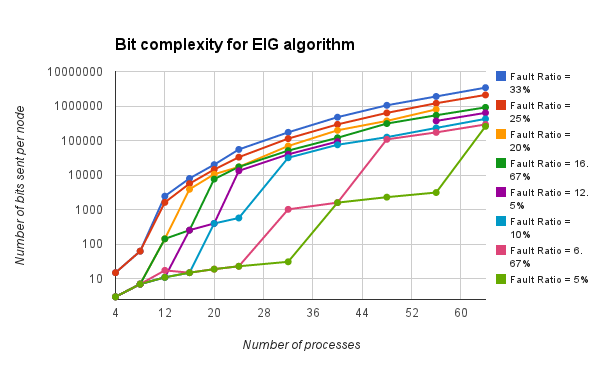
\includegraphics[scale=0.4]{eig}
\caption{Consensus results for EIG algorithm}
 \label{fig:eig}
\end{figure}

For the Pull-Push algorithm, as the network size increases the bit complexity displays a polylogarithmic growth. The growth trend is similar for all fault ratios for small and larger networks. The increase in number of faults has no tremendous effect on the number of bits sent per node, which implies that message complexity of these algorithms is not influenced by the number of faults. This is can be attributed to the fact that in the protocol, even if byzantine nodes try to send conflicting values and arbitrary number of them to samplers for the purpose of flooding, the samplers do not receive enough of them to forward these messsages further in the protocol. This can be see from Figs. \ref{fig:pull_push}.
\begin{figure}[h]
 \centering
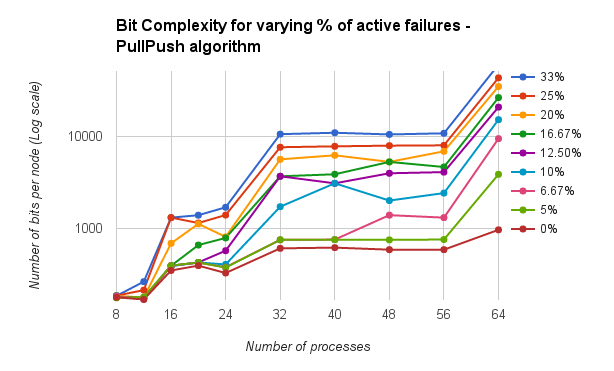
\includegraphics[scale=0.4]{pull_push}
\caption{Consensus results for Pull-Push algorithm}
 \label{fig:pull_push}
\end{figure}

\begin{figure}[h]
 \centering
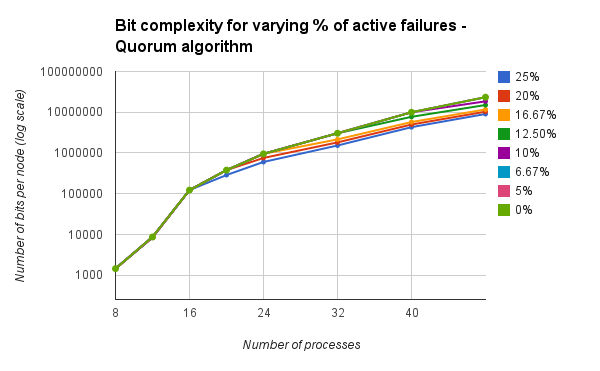
\includegraphics[scale=0.4]{quorum}
\caption{Consensus results for Quorum algorithm}
 \label{fig:quorum}
\end{figure}

\subsubsection{Comparison}
As can be seen from Fig. \ref{fig:comp}, for large networks $n > 64$, on varying the ratio of faults to the number of processes, i.e., $f/n$ lies in the range $[0, 1/3)$ for algorithms EIG and Pull-Push and in the range $[0, 1/4)$ for algorithm Quorum, the algorithm Pull-Push performs much better, than the other algorithms. For this algorithm, the change in the ratio does not affect the complexity much, whereas for algorithm EIG we can see a slight increase. This is due to byzantine nodes trying to send $O(n^2)$ bits to every node in every round and good nodes having to send the complete byzantine list in every round. We modify this protocol a little and require that instead of sending the complete byzantine list every time, only the changes to this list be sent in every round. This would overall reduce communication bits as good nodes would send a bit for every node only if it was newly added to the byzantine list at the end of the previous round. This modified version of the algorithm performs much better and even though the communication bits are high for small fault ratios it reduces the communication complexity by $O(n)$. 
\begin{figure}[h]
 \centering
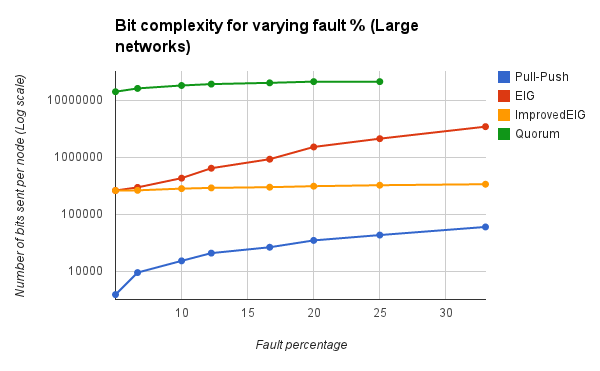
\includegraphics[scale=0.4]{LargeNetBit}
\caption{Comparison for large networks}
 \label{fig:comp}
\end{figure}

\begin{figure}[h]
 \centering
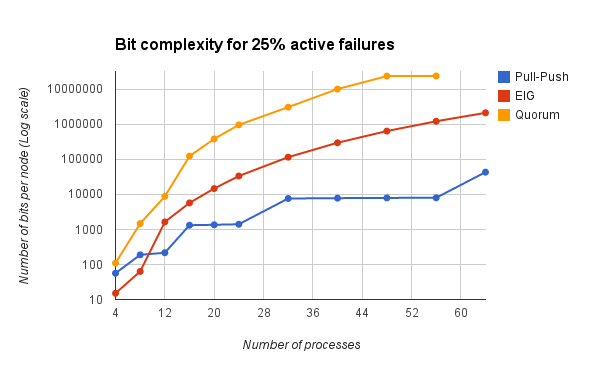
\includegraphics[scale=0.4]{Fault25}
\caption{ Comparison for variable number of faults in each algorithm}
 \label{fig:fault25}
\end{figure}

\begin{figure}[h]
 \centering
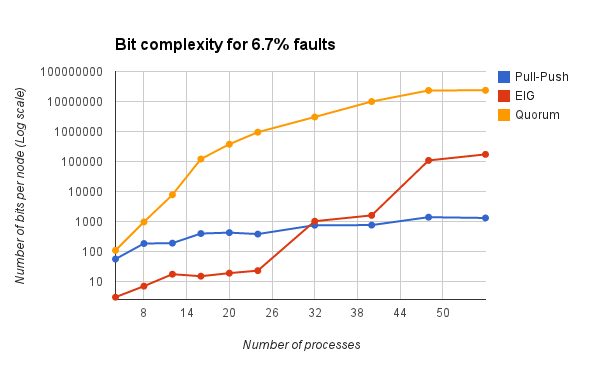
\includegraphics[scale=0.4]{Fault667}
\caption{ Comparison for variable number of faults in each algorithm}
 \label{fig:fault667}
\end{figure}

\begin{figure}[h]
 \centering
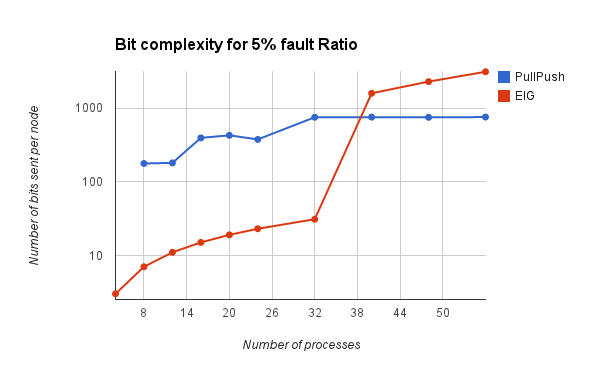
\includegraphics[scale=0.4]{Fault5}
\caption{ Comparison for variable number of faults in each algorithm}
 \label{fig:fault5}
\end{figure}

For small networks ($n < 48$), if the fault ratio is small and in the range $[0, 1/15)$, Figs. \ref{fig:fault667} and \ref{fig:fault5} show that algorithm EIG performs much better than any of the other algorithms. This is simply because only the first three rounds of this algorithm will be executed and since the ratio is small, a simple broadcast is sufficient to gather all the information. Pull-Push and Quorum, more complex algorithms perform worse in such scenarios.

Depending on the system requirements such as how fast we want the information to reach the destination, bandwidth and so on, there were two mechanisms we used to send the messages. In an algorithm like Pull-Push, where multiple message packets maybe sent to the same node by a process in the same round, one could marshall all the packets into one packet and then send it. This obviously comes at the cost parallelization where one has to first wait to receive all messages from previous round, perform operations and then send out messages all at once. The latter method requires sending more number of packets, whereas the former method implies that only one packet will be sent in each broadcast. Although, the number of bits sent remains the same. %The difference in the number of messages sent for the two mechanisms can be seen in Fig. \ref{fig:opt}.
%\begin{figure}[h]
% \centering
%\includegraphics[scale=0.55]{optimized}
%\caption{ EIG algorithm when messages are grouped before sending}
% \label{fig:opt}
%\end{figure}


\subsection{Time Complexity}

For comparison of time complexity we compare the CPU times required for the execution of each algorithm.  From figures \ref{fig:time6} and \ref{fig:time16} we see that CPU time utilisation for EIG, for small fault ratios, closely follows Pull-Push CPU time utilisation even as the size of the network increases. This is due to the less number of rounds executed by EIG at these ratios. For higher ratios, Pull-Push clearly performs better.

\begin{figure}[h]
 \centering
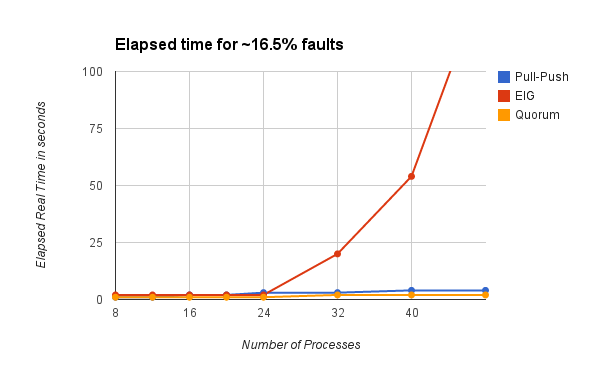
\includegraphics[scale=0.4]{Time16}
\caption{Time Complexity comparison}
 \label{fig:time16}
\end{figure}

\begin{figure}[h]
 \centering
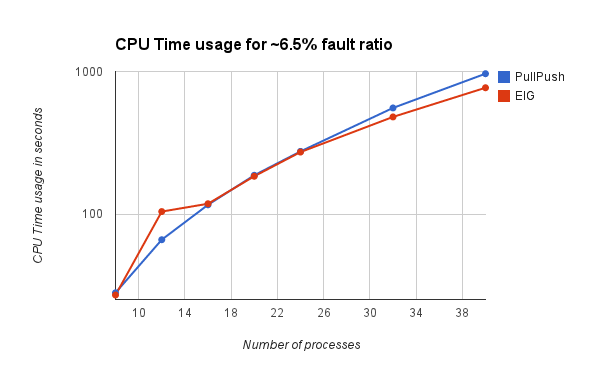
\includegraphics[scale=0.4]{Time6}
\caption{Time Complexity comparison}
 \label{fig:time6}
\end{figure}

\subsection{Round Complexity}
Round complexity is the number of phases that have to be executed sequentially by a processes and one cannot parallelize these phases. For example, in algorithm EIG, a round consists of broadcast of messages at the same level $i$ in the EIG trees by each process. For algorithm Quorum, a round consists of broadcast of messages during a particular subprotocol. There are two outlooks to analyzing the round complexity of this algorithm. The first is that each of the subprotocols $S_i^j$ could be executed in parallel since none of these subprotocols are dependent on each other. Hence, all of them together make one round. But, parallel execution of these subprotocols is not possible due to resource constraints then each of them is an independent round. For algorithm Pull-Push, the push phase makes one round and sending, routing and answering in the pull phase form imdependent rounds.

A comparison of the round complexities can be seen in Figs. \ref{fig:round6} and \ref{fig:round16} for fault percentage $~6.5\%$ and $~16.5\%$, respectively. In both the figures parallel execution of subprotocols for algorithm Quorum is assumed. 

\begin{figure}[h]
 \centering
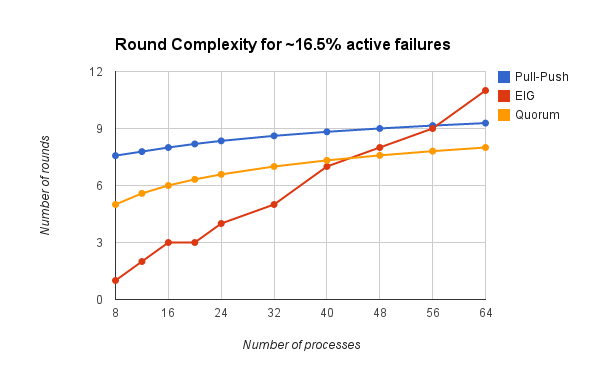
\includegraphics[scale=0.4]{Round16}
\caption{Time Complexity comparison}
 \label{fig:round16}
\end{figure}

\begin{figure}[h]
 \centering
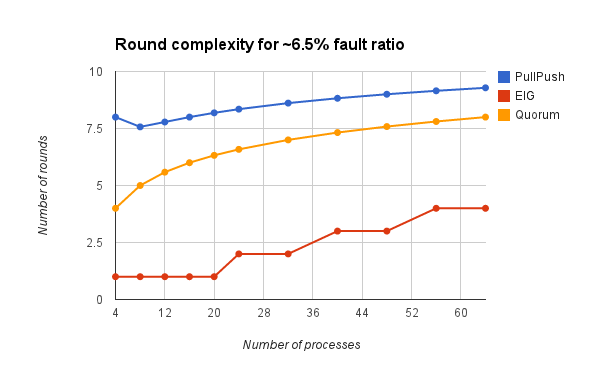
\includegraphics[scale=0.4]{Round6}
\caption{Time Complexity comparison}
 \label{fig:round6}
\end{figure}
%Fig. \ref{fig:time} the first mechanism for calculating time complexity of algorithm Quorum is used, where it is considered that all the subprotocols together form one round. This figure shows the algorithm Quorum gives better performance than algorithms EIG and Pull-Push as the number of processes in the network increases. Also, algorithm Pull-Push diverges in complexity due to increasing number of candidate strings that could be injected by the adversarial processes.

%Fig. \ref{fig:time_nopar}, shows a comparison of time complexities if each subprotocol in algorithm Quorum is treated as an individual round. In contrast to Fig. \ref{fig:time}, this figure clearly shows that the time complexity of algorithm Quorum increases rapidly, whereas for algorithms EIG and Pull-Push there is no drastic increase. Hence, if resources are limited and parallel processing of each subprotocol is not possible, algorithm Quorum does not give good performance.
%
%\begin{figure}[h]
% \centering
%\includegraphics[scale=0.55]{time_nopar}
%\caption{Time Complexity comparison no parallel execution}
% \label{fig:time_nopar}
%\end{figure}


\subsection{Discussion}

In real-world applications, achieving distributed consensus has become essential. In most cases, consensus is only a small but frequently used sub-component of a larger protocol such as in distributed databases. Thus, improving the message and time complexity of this algorithm is essential to the overall performance of such systems. Also, one needs to consider implementation issues that come along with any of these algorithms and not only their theoretical results. During implementation, one can even improve certain tasks such as sending a larger message instead of many smaller messages or executing parallelizable tasks at the same time on multi-core machines.  

As can be seen from the figures above, according to the requirements and resources available, each algorithm gives us different performance. Once we have an algorithm to implement, the first thing to consider before implementation is what resources we have and how can we design the system such that we get optimal results for the available resources. Although the testbed framework was implemented and run on a single machine, it was crucial for us to use as less TCP connections at a time as possible. Therefore, we marshalled all individual messages, in a round, into one single message before broadcasting. We report on results for number of messages sent if each individual message had been sent separately, since either of the methods do not affect the total number of bits transferred. Another optimization that would have saved the running time of the system would have been to use UDP connections instead of TCP since they take up less resources and provide lesser overhead. Even though UDP connections do not guarantee message delivery, for a local system it could have been considered highly reliable still. The rationale behind using TCP connections for this testbed framework was to model and understand implementation issues for more realistic distributed applications, which could have peers separated by geographical distance. In such cases, TCP connections provide greater reliability. 

An analysis of the three algorithms and their performance for a wide range of number of processes and faults shows that communication of each process with as few honest processes as possible will yield good results. As this inhibits byzantine processes from influencing values of every other process. The use of randomly chosen quorums to filter requests gave us good results as can be seen in algorithm Pull-Push. Also, the use of parallelization of subtasks in the case of algorithm Quorum, gave good time complexity results. The combined use of these two techniques might help us design improved algorithms in the future to solve the problem of distributed consensus. 




